\section{Phân tích và thiết kế hệ thống}

\subsection{Xác định các bên liên quan và tác nhân hệ thống}

Trong một hệ thống mạng xã hội học đường tích hợp AI và Bản đồ số, việc xác định rõ thực thể tham gia giúp định hình phạm vi thiết kế và các luồng xử lý dữ liệu (đặc biệt là dữ liệu cá nhân và điểm rèn luyện). 

\subsubsection{Các bên liên quan (Stakeholders}

Stakeholders là những cá nhân hoặc tổ chức có lợi ích trực tiếp hoặc gián tiếp từ sự thành công của dự án:

\begin{itemize}
    \item Ban Giám hiệu và Nhà trường: Đóng vai trò là đơn vị quản lý vĩ mô. Nhà trường quan tâm đến việc tạo ra một môi trường tương tác an toàn, lành mạnh cho sinh viên, đồng thời ứng dụng công nghệ để hiện đại hóa công tác quản lý hoạt động phong trào.

    \item Đội ngũ phát triển (Developers): Chịu trách nhiệm về mặt kỹ thuật, đảm bảo sự ổn định của hệ thống vận hành trên Docker, tối ưu hóa các câu lệnh truy vấn không gian và duy trì độ chính xác của trợ lý AI.
    
    \item Đoàn thanh niên và Hội sinh viên: Là đơn vị trực tiếp điều phối các hoạt động ngoại khóa. Họ cần một công cụ trực quan để thông tin đến sinh viên nhanh nhất và quản lý dữ liệu tham gia một cách minh bạch.
\end{itemize}

\subsection{Các tác nhân hệ thống (Actors)}

Tác nhân là những thực thể tương tác trực tiếp với các chức năng của UniConnect. Hệ thống được thiết kế với 4 nhóm tác nhân sau:

\begin{enumerate}
    \item \textbf{Tác nhân Sinh viên (Student):}
    Là nhóm tác nhân trung tâm, sinh viên tương tác với hệ thống nhằm mục đích kết nối xã hội và hỗ trợ học tập. Các tương tác chính bao gồm:
    \begin{itemize}
        \item Quản lý hiện diện: Cập nhật vị trí hiện tại trên bản đồ khuôn viên trường, thiết lập trạng thái cá nhân (đang học, đang nghỉ, cần tìm bạn học nhóm) hoặc chọn chế độ ẩn danh.
        
        \item Tương tác hoạt động tự phát: Khởi tạo các điểm ghim hoạt động trên bản đồ (ví dụ: rủ chơi thể thao, học nhóm tại thư viện); tham gia hoặc rời khỏi các hoạt động của người khác.
        
        \item Quản lý tri thức: Đăng tải các tài liệu học thuật cá nhân (giáo trình, đề thi cũ); đặt câu hỏi và thảo luận trong cộng đồng (Q\&A).
        
        \item Khai thác AI: Đặt câu hỏi cho Trợ lý ảo để tra cứu nhanh thông tin trường học hoặc yêu cầu gợi ý các tài liệu/hoạt động phù hợp với năng lực cá nhân.
    \end{itemize}

    \item \textbf{Tác nhân Cán bộ trường / Ban tổ chức (Staff/Organizer)}
    Đây là tác nhân mở rộng của Sinh viên nhưng có thêm các quyền hạn quản lý cấp cao để phục vụ công tác tổ chức chính quy. Các tương tác đặc thù bao gồm:
    \begin{itemize}
        \item Tổ chức hoạt động chính quy: Khởi tạo các sự kiện có gắn kèm thuộc tính "Điểm rèn luyện", "Ngày công tác xã hội" hoặc "Hội thảo học thuật". Các hoạt động này sẽ được ưu tiên hiển thị nổi bật trên bản đồ.

        \item Quản lý danh sách thành viên: Theo dõi số lượng và danh tính sinh viên đăng ký tham gia hoạt động theo thời gian thực.
        
        \item Khai thác dữ liệu định danh: Trích xuất báo cáo danh sách thành viên tham gia dưới định dạng tệp tin (Excel/CSV) bao gồm Email và Mã số sinh viên để phục vụ việc cộng điểm rèn luyện sau sự kiện.
        
        \item Điều phối truyền thông: Gửi thông báo nhắc hẹn hoặc cập nhật thay đổi thông tin hoạt động tới toàn bộ sinh viên đã đăng ký tham gia.
    \end{itemize}

    \item \textbf{Tác nhân Quản trị viên (Admin)}
    Đóng vai trò duy trì sự ổn định và an toàn của toàn bộ hệ thống. Các tương tác tập trung vào quản lý kỹ thuật:
    \begin{itemize}
        \item Quản lý định danh: Phê duyệt hoặc khóa tài khoản người dùng vi phạm quy định; quản lý quyền hạn của các tài khoản thuộc nhóm Cán bộ trường.

        \item Kiểm soát nội dung (Moderation): Giám sát các hoạt động và tài liệu bị người dùng báo cáo; trực tiếp gỡ bỏ các thông tin sai lệch, không lành mạnh khỏi bản đồ và diễn đàn.
        
        \item Vận hành hạ tầng: Theo dõi trạng thái của các Container trong Docker; cập nhật kho dữ liệu tri thức (Knowledge Base) để trợ lý AI luôn có thông tin mới nhất.
        
        \item Thống kê hệ thống: Xem báo cáo về mật độ hoạt động của sinh viên trong campus theo thời gian để tư vấn cho nhà trường về việc phân bổ không gian học tập.
    \end{itemize}

    \item \textbf{Tác nhân Trợ lý ảo AI (System Actor)}
    Là một thực thể phần mềm thông minh, thực hiện các tương tác tự động nhằm tối ưu hóa trải nghiệm cho các tác nhân còn lại:
    \begin{itemize}
        \item Xử lý dữ liệu nhúng (Embedding): Tự động chuyển đổi các bài đăng, tài liệu và hồ sơ người dùng thành các vector toán học ngay khi dữ liệu được tạo mới.

        \item Hỗ trợ truy xuất (Retrieval): Lắng nghe các yêu cầu tìm kiếm ngữ nghĩa và trả về kết quả dựa trên độ tương đồng về sở thích hoặc nội dung học tập.
        
        \item Hỗ trợ tư vấn (RAG): Tổng hợp dữ liệu từ cơ sở dữ liệu nội bộ để cung cấp các câu trả lời chính xác, mang tính cá nhân hóa cho từng sinh viên thông qua giao diện chat.
    \end{itemize}
\end{enumerate}

\subsection{Yêu cầu chức năng (Functional requirements}

\subsubsection{Nhóm chức năng dành cho Sinh viên (Student)}
\begin{itemize}
    \item Quản lý tài khoản: Đăng ký, đăng nhập, cập nhật hồ sơ cá nhân (chuyên ngành, khóa học, sở thích).

    \item Tương tác bản đồ số: 
    \begin{itemize}
        \item Xem vị trí các điểm hoạt động đang diễn ra.
    
        \item Chia sẻ vị trí hiện tại hoặc thiết lập trạng thái ẩn danh/hiện diện.
    \end{itemize}
    
    \item Quản lý hoạt động tự phát:
    \begin{itemize}
        \item Tạo hoạt động học tập, thể thao, giải trí tại một vị trí cụ thể trên bản đồ.
    
        \item Đăng ký tham gia hoặc hủy tham gia các hoạt động do người khác khởi tạo.
    \end{itemize}
    
    \item Diễn đàn và Tài liệu:
    \begin{itemize}
        \item Đăng tải tài liệu (PDF, Slide, hình ảnh) và phân loại theo môn học.
    
        \item Đặt câu hỏi, trả lời và tham gia thảo luận trong các chủ đề học thuật.
        
        \item Đánh giá chất lượng tài liệu và câu trả lời thông qua cơ chế Upvote/Downvote.
    \end{itemize}
    
    \item Hỗ trợ AI: Gửi yêu cầu tư vấn, hỏi đáp về thông tin nhà trường và tìm kiếm tài liệu thông qua giao diện Chatbot.
\end{itemize}


\subsubsection{Nhóm chức năng dành cho Cán bộ trường / Ban tổ chức (Staff/Organizer)}
\begin{itemize}
    \item Tổ chức sự kiện chính thống: 
    \begin{itemize}
        \item Tạo các hoạt động có tính chất đặc biệt như: Hội thảo, Ngày hội việc làm, Hoạt động tình nguyện.
    
        \item Gắn thuộc tính "Cộng điểm rèn luyện" hoặc "Ngày công tác xã hội" cho sự kiện.
    \end{itemize}
    
    \item Quản lý người tham gia:
    \begin{itemize}
        \item Phê duyệt danh sách sinh viên đăng ký (đối với các sự kiện giới hạn số lượng).
    
        \item Gửi thông báo (Push notification/Email) đến toàn bộ sinh viên trong sự kiện.
    \end{itemize}
    
    \item Trích xuất dữ liệu:
    \begin{itemize}
        \item Xuất báo cáo: Trích xuất danh sách sinh viên đã tham gia hoạt động ra tệp tin định dạng Excel/CSV.
    
        \item Dữ liệu định danh: Tiếp cận địa chỉ Email và Mã số sinh viên của người tham gia để phục vụ việc xác nhận quyền lợi cho sinh viên.
    \end{itemize}
\end{itemize}


\subsubsection{Nhóm chức năng dành cho Quản trị viên (Admin)}

\begin{itemize}
    \item Quản lý người dùng: Kích hoạt, khóa tài khoản hoặc thay đổi vai trò người dùng (nâng cấp từ Sinh viên lên Cán bộ trường).

    \item Kiểm duyệt nội dung (Moderation): 
    \begin{itemize}
        \item Tiếp nhận và xử lý các báo cáo vi phạm từ cộng đồng.
    
        \item Xóa bỏ các bài đăng, tài liệu hoặc điểm ghim hoạt động có nội dung không phù hợp.
    \end{itemize}
    
    \item Quản lý kho tri thức AI: Cập nhật các tệp tin quy định, hướng dẫn của nhà trường vào cơ sở dữ liệu Vector để AI học thông tin mới.
    
    \item Báo cáo hệ thống: Xem thống kê về lượng truy cập, mật độ hoạt động trên bản đồ và các chủ đề thảo luận sôi nổi nhất.
\end{itemize}

\subsubsection{Nhóm chức năng của Trợ lý ảo AI (System Actor)}

\begin{itemize}
    \item Xử lý ngôn ngữ tự nhiên: Phân tích ý định (Intent) từ câu hỏi của sinh viên để đưa ra phản hồi phù hợp.

    \item Truy xuất thông tin (RAG): Tìm kiếm và tổng hợp thông tin từ kho dữ liệu nội bộ để trả lời các câu hỏi về thủ tục, quy định trường học.
    
    \item Gợi ý thông minh: Tự động đề xuất các hoạt động hoặc bạn bè có độ tương đồng về sở thích/ngành học dựa trên thuật toán tìm kiếm Vector.
\end{itemize}

\subsection{Yêu cầu phi chức năng (Non-functional requirements}

\subsubsection{Yêu cầu về hiệu năng và khả năng đáp ứng (Performance)} 
\begin{itemize}
    \item Tốc độ xử lý Vector: Thời gian để hệ thống thực hiện nhúng (Embedding) một đoạn văn bản và tìm kiếm các kết quả tương đồng trong cơ sở dữ liệu pgvector không được vượt quá 300ms.

    \item Độ trễ cập nhật bản đồ: Khi một "Hoạt động" được tạo mới hoặc vị trí sinh viên thay đổi, thông tin phải được đồng bộ hóa tới các máy trạm khác trong vòng dưới 1 giây.

    \item Tối ưu hóa băng thông: Các dữ liệu bản đồ (Tiles) và dữ liệu địa lý (GeoJSON) phải được nén hoặc lưu vào bộ nhớ đệm (Cache) ở phía Client để giảm thiểu lưu lượng mạng khi di chuyển trong khu vực sóng yếu.
\end{itemize}


\subsubsection{Yêu cầu về tính tin cậy và khả năng phục hồi (Reliability)} 
\begin{itemize}
    \item Tính toàn vẹn dữ liệu: Hệ thống phải đảm bảo không mất dữ liệu khi xảy ra sự cố đột ngột của các Container Backend. Sử dụng cơ chế Docker Volumes để lưu trữ dữ liệu PostgreSQL tách biệt khỏi vòng đời của Container.

    \item Khả năng chịu lỗi: Trong trường hợp dịch vụ AI (như OpenAI API hoặc mô hình Local) bị gián đoạn, các chức năng cơ bản của hệ thống như xem bản đồ và đăng bài vẫn phải hoạt động bình thường (Graceful Degradation).
\end{itemize}


\subsubsection{Yêu cầu về bảo mật và quyền riêng tư chuyên sâu} 
\begin{itemize}
    \item Phân quyền đa tầng: * Tầng dữ liệu: Sinh viên tuyệt đối không thể truy cập trực tiếp vào các hàm trích xuất Email/MSSV của hệ thống.

    \item Tầng API: Mọi yêu cầu từ Frontend phải đi kèm mã xác thực JWT (JSON Web Token) có thời hạn.

    \item Xử lý dữ liệu nhạy cảm: Vị trí của sinh viên chỉ được lưu trữ dưới dạng tọa độ làm tròn khi không ở trong trạng thái "Chia sẻ công khai" để tránh việc bị theo dõi ngoài ý muốn.

    \item Ghi vết (Audit Logging): Hệ thống phải ghi lại lịch sử các thao tác thay đổi dữ liệu quan trọng như: Admin xóa bài, Cán bộ xuất danh sách email, hoặc thay đổi quyền hạn người dùng.
\end{itemize}


\subsubsection{Yêu cầu về khả năng mở rộng và bảo trì (Scalability)} 
\begin{itemize}
    \item Kiến trúc Micro-services ready: Các thành phần được đóng gói riêng biệt bằng Docker Compose, cho phép dễ dàng tách riêng Database hoặc AI Worker ra các máy chủ độc lập khi số lượng sinh viên tăng lên (ví dụ: mở rộng cho toàn bộ các cơ sở của trường).

    \item Tiêu chuẩn mã nguồn: Mã nguồn phải tuân thủ các quy tắc Linting (cho TypeScript) và PEP8 (cho Python) để phục vụ việc bảo trì, nâng cấp bởi đội ngũ khác trong tương lai.
\end{itemize}


\subsubsectionautorefname{Yêu cầu về tính chính xác và đạo đức AI (AI Ethics)}
\begin{itemize}
    \item Độ chính xác của RAG: Câu trả lời của Trợ lý ảo phải dựa trên ít nhất 80\% dữ liệu từ kho tri thức nội bộ. Nếu không tìm thấy thông tin, AI phải trả lời "Tôi không biết" thay vì tự dự đoán thông tin sai lệch.

    \item Kiểm soát nội dung độc hại: Hệ thống nhúng (Embedding) cần có bộ lọc để nhận diện và cảnh báo các nội dung nhạy cảm, vi phạm thuần phong mỹ tục ngay khi sinh viên đăng tải.
\end{itemize}

\subsection{Use case diagram tổng quát}

\begin{figure}[H]
    \centering
    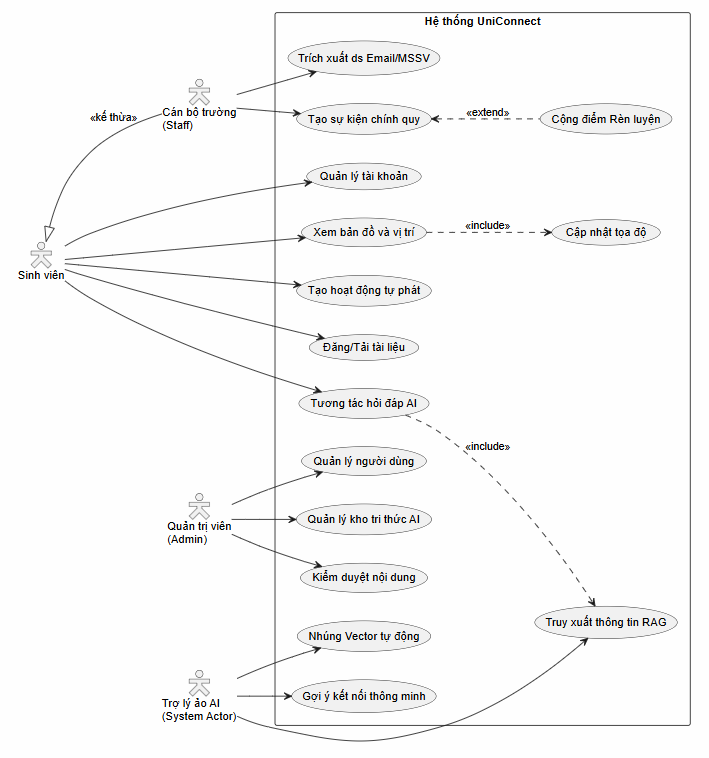
\includegraphics[width=0.85\textwidth]{Images/use-case-tong-quat.png}
    \caption{Sơ đồ Use Case tổng quát hệ thống UniConnect}
    \label{fig:usecase_tongquat}
\end{figure}

\subsection{Đặc tả Use case}
\subsubsection{Tạo hoạt động trên bản đồ}

\begin{figure}[H]
    \centering
    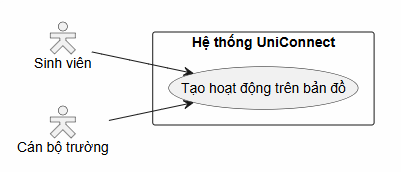
\includegraphics[width=0.85\textwidth]{Images/use-case-tao-hoat-dong.png}
    \caption{Sơ đồ Use Case tạo hoạt động}
    \label{fig:usecase_tao_hoat_dong}
\end{figure}

\renewcommand{\arraystretch}{1.5} % Tăng khoảng cách giữa các dòng cho dễ nhìn
\begin{xltabular}{\textwidth}{|>{\bfseries}p{3.5cm}|X|}
    % Cấu hình Tiêu đề và Nhãn bảng
    \caption{Đặc tả Use case Tạo hoạt động trên bản đồ} \label{tab:uc_taohoatdong} \\
    \hline
    \endfirsthead
    \caption[]{Đặc tả Use case Tạo hoạt động trên bản đồ} \\
    \hline
    \endhead
    \hline
    \endfoot
    \hline
    \endlastfoot

    % Nội dung bảng
    Use case name & Tạo hoạt động trên bản đồ \\ \hline
    Actor & Sinh viên, Cán bộ trường \\ \hline
    Description & Cho phép người dùng khởi tạo một điểm ghim (Marker) đại diện cho một sự kiện hoặc hoạt động (học nhóm, thể thao, sự kiện khoa) tại một tọa độ cụ thể trên khuôn viên trường. \\ \hline
    Preconditions & Người dùng đã đăng nhập thành công vào hệ thống và cấp quyền truy cập vị trí cho trình duyệt/ứng dụng. \\ \hline
    Postconditions & Hệ thống lưu thông tin hoạt động vào cơ sở dữ liệu, tự động nhúng vector mô tả hoạt động và hiển thị điểm ghim mới lên bản đồ cho tất cả người dùng khác. \\ \hline
    
    % Phân rã Normal Flow để hỗ trợ ngắt trang
    \textbf{Normal Flow} & 1. Actor nhấn giữ (long-press) vào một vị trí cụ thể trên giao diện bản đồ. \\
    & 2. Hệ thống hiển thị biểu mẫu yêu cầu nhập thông tin hoạt động. \\ 
    & 3. Actor nhập dữ liệu: Tiêu đề, Mô tả, Thời gian bắt đầu và Số lượng giới hạn. \\ 
    & 4. Actor nhấn nút "Tạo hoạt động". \\ 
    & 5. Hệ thống gửi dữ liệu tọa độ và nội dung form lên Backend xử lý. \\ 
    & 6. Hệ thống lưu bản ghi vào CSDL và chạy ngầm tác vụ nhúng Vector cho phần mô tả. \\ 
    & 7. Hệ thống thông báo tạo thành công và tải lại lớp bản đồ để hiển thị Marker mới. \\ \hline
    
    Alternative flow & Actor bỏ trống các trường thông tin bắt buộc (Tiêu đề, Thời gian); hệ thống sẽ chặn việc gửi dữ liệu ở phía Frontend, hiển thị viền đỏ ở các ô nhập liệu và yêu cầu điền đầy đủ. \\ \hline
    Exception & Sự cố đường truyền hoặc hết phiên đăng nhập: Tại bước 5, nếu thiết bị mất mạng hoặc token JWT đã hết hạn, máy chủ sẽ không thể xử lý. Hệ thống hiển thị thông báo "Kết nối thất bại, vui lòng thử lại", đồng thời giữ nguyên các thông tin Actor đã nhập trên biểu mẫu để tránh mất dữ liệu. \\ \hline

\end{xltabular}

\subsubsection{Quản lý hoạt động}

\begin{figure}[H]
    \centering
    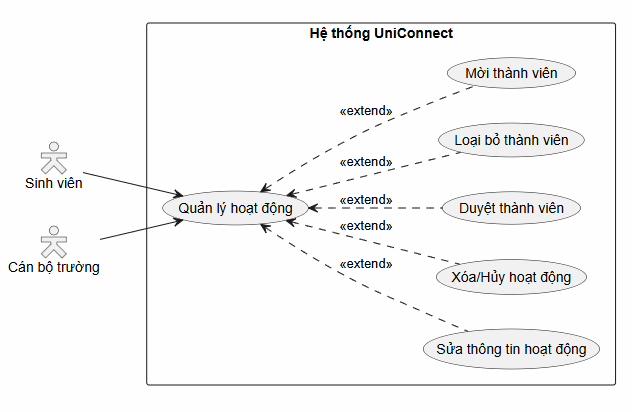
\includegraphics[width=0.85\textwidth]{Images/use-case-quan-ly-hoat-dong.png}
    \caption{Sơ đồ Use Case quản lý hoạt động}
    \label{fig:usecase_quan_ly_hoat_dong}
\end{figure}

\renewcommand{\arraystretch}{1.5} % Tăng khoảng cách dòng cho thoáng bảng
\begin{xltabular}{\textwidth}{|>{\bfseries}p{3.5cm}|X|}
    % Cấu hình Tiêu đề và Nhãn bảng (Tự động lặp lại tiêu đề nếu sang trang mới)
    \caption{Đặc tả Use case Quản lý hoạt động} \label{tab:uc_quanlyhoatdong} \\
    \hline
    \endfirsthead
    \caption[]{Đặc tả Use case Quản lý hoạt động} \\
    \hline
    \endhead
    \hline
    \endfoot
    \hline
    \endlastfoot

    % Kịch bản chi tiết bắt đầu từ đây
    Use case name & Quản lý hoạt động \\ \hline
    Actor & Sinh viên, Cán bộ trường (Chủ sở hữu hoạt động) \\ \hline
    Description & Cho phép người dùng quản lý các hoạt động hoặc sự kiện do chính mình khởi tạo trên bản đồ, bao gồm việc cập nhật thông tin, hủy hoạt động và điều phối danh sách thành viên tham gia. \\ \hline
    Preconditions & Actor đã đăng nhập thành công và hệ thống xác thực Actor chính là chủ sở hữu (người tạo) của hoạt động đó. \\ \hline
    Postconditions & Các thay đổi về thông tin hoạt động hoặc trạng thái thành viên được cập nhật đồng bộ vào cơ sở dữ liệu. \\ \hline
    
    % Bắt đầu phân rã hàng cho Normal Flow để tạo điểm ngắt trang
    \textbf{Normal Flow} & 1. Actor truy cập vào mục "Hoạt động của tôi" và chọn hoạt động cần điều phối. \\
    & 2. Hệ thống hiển thị bảng điều khiển quản lý (Dashboard) của hoạt động đó. \\ 
    & 3. Actor lựa chọn thực hiện một trong các nhánh hành động sau:
    \vspace{0.2cm}
    \begin{itemize}[leftmargin=*, noitemsep]
        \item \textbf{Nhánh Sửa thông tin:} Actor chọn "Chỉnh sửa", thay đổi các thông tin (Tiêu đề, Mô tả, Số lượng) và nhấn "Cập nhật". Hệ thống kiểm tra dữ liệu và lưu vào CSDL.
        \item \textbf{Nhánh Xóa/Hủy:} Actor chọn "Hủy hoạt động", hệ thống hiển thị hộp thoại cảnh báo. Actor nhấn "Xác nhận", hệ thống chuyển trạng thái sang "Đã hủy" và gỡ điểm ghim khỏi bản đồ.
        \item \textbf{Nhánh Duyệt thành viên:} Trong tab "Yêu cầu", Actor nhấn "Chấp nhận" đối với các sinh viên đang chờ. Hệ thống chuyển trạng thái của họ thành thành viên chính thức.
        \item \textbf{Nhánh Loại bỏ thành viên:} Trong tab "Thành viên", Actor chọn một sinh viên và nhấn "Loại bỏ khỏi nhóm". Hệ thống xóa sinh viên đó khỏi danh sách tham gia.
        \item \textbf{Nhánh Mời thành viên:} Actor nhập Mã số sinh viên/Email của người cần mời và nhấn "Gửi lời mời". Hệ thống gửi thông báo mời tham gia tới tài khoản mục tiêu.
    \end{itemize} \\ 
    & 4. Hệ thống hiển thị thông báo "Thao tác thành công" và cập nhật lại giao diện Dashboard. \\ \hline
    
    % Các mục cuối bảng
    Alternative flow & Tại bước 3, nếu Actor đang thực hiện dở dang một thao tác (ví dụ đang sửa thông tin hoặc đang mở hộp thoại xóa) nhưng nhấn nút "Quay lại" hoặc đóng tab, hệ thống sẽ hủy bỏ toàn bộ các thay đổi chưa lưu và quay về giao diện bước 2. \\ \hline
    Exception & Hoạt động đã bị khóa: Tại bước 1, nếu hoạt động này vừa bị Admin ẩn hoặc khóa do vi phạm nội dung ngay trước đó, hệ thống sẽ từ chối quyền truy cập, hiển thị thông báo "Hoạt động không còn khả dụng" và đưa Actor về trang chủ. \\ \hline

\end{xltabular}

\subsubsection{Tương tác với hoạt động}

\begin{figure}[H]
    \centering
    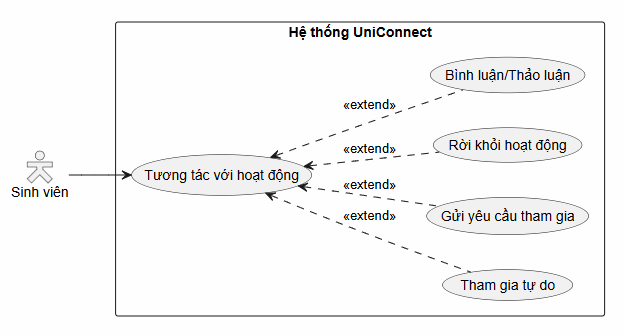
\includegraphics[width=0.85\textwidth]{Images/use-case-tuong-tac-hoat-dong.png} 
    \caption{Sơ đồ Use Case tham gia và tương tác hoạt động}
    \label{fig:usecase_tuong_tac_hoat_dong}
\end{figure}

\renewcommand{\arraystretch}{1.5}
\begin{xltabular}{\textwidth}{|>{\bfseries}p{3.5cm}|X|}
    % Cấu hình Tiêu đề và Nhãn bảng
    \caption{Đặc tả Use case Tham gia và tương tác hoạt động} \label{tab:uc_tuongtachoatdong} \\
    \hline
    \endfirsthead
    \caption[]{Đặc tả Use case Tham gia và tương tác hoạt động} \\
    \hline
    \endhead
    \hline
    \endfoot
    \hline
    \endlastfoot

    % Nội dung bảng
    Use case name & Tham gia và tương tác hoạt động \\ \hline
    Actor & Sinh viên \\ \hline
    Description & Cho phép Sinh viên tham gia vào các hoạt động trên bản đồ (có thể vào trực tiếp hoặc cần phê duyệt), rời khỏi hoạt động khi đổi ý, và thảo luận/bình luận bên trong không gian của hoạt động đó. \\ \hline
    Preconditions & Sinh viên đã đăng nhập hệ thống. Hoạt động mục tiêu đang trong trạng thái "Đang diễn ra" hoặc "Sắp diễn ra" (chưa kết thúc/chưa bị khóa). \\ \hline
    Postconditions & Trạng thái tham gia của Sinh viên được cập nhật (Đã tham gia/Đang chờ/Đã rời). Các bình luận (nếu có) được lưu vào cơ sở dữ liệu và hiển thị công khai cho những người xem hoạt động. \\ \hline
    
    % Phân rã Normal Flow để hỗ trợ ngắt trang
    \textbf{Normal Flow} & 1. Sinh viên nhấn vào một điểm ghim hoạt động trên giao diện bản đồ. \\ 
    & 2. Hệ thống hiển thị bảng thông tin chi tiết của hoạt động (Mô tả, Danh sách thành viên, Khu vực thảo luận). \\ 
    & 3. Tùy thuộc vào thiết lập của hoạt động và trạng thái hiện tại của Sinh viên, Sinh viên thực hiện một trong các nhánh sau:
    \vspace{0.2cm}
    \begin{itemize}[leftmargin=*, noitemsep]
        \item \textbf{Nhánh Tham gia tự do:} (Hoạt động không yêu cầu duyệt). Sinh viên nhấn "Tham gia". Hệ thống lập tức thêm Sinh viên vào danh sách thành viên chính thức.
        \item \textbf{Nhánh Xin tham gia:} (Hoạt động yêu cầu phê duyệt). Sinh viên nhấn "Xin tham gia". Hệ thống ghi nhận trạng thái "Đang chờ duyệt" và gửi thông báo (Notification) đến chủ sở hữu hoạt động.
        \item \textbf{Nhánh Rời khỏi:} Sinh viên (đang là thành viên hoặc đang chờ duyệt) nhấn nút "Rời khỏi". Hệ thống yêu cầu xác nhận, sau đó xóa Sinh viên khỏi danh sách tham gia.
        \item \textbf{Nhánh Bình luận:} Sinh viên nhập nội dung vào ô thảo luận và nhấn "Gửi". Hệ thống lưu bình luận vào CSDL và tự động cập nhật hiển thị lên luồng thảo luận.
    \end{itemize} \\ 
    & 4. Hệ thống hiển thị thông báo "Thao tác thành công" (hoặc "Đã gửi yêu cầu") và tải lại giao diện chi tiết hoạt động để cập nhật dữ liệu mới nhất. \\ \hline
    
    Alternative flow & Ở nhánh Bình luận, nếu Sinh viên chỉ nhập các khoảng trắng hoặc để trống ô nội dung, hệ thống (Frontend) sẽ vô hiệu hóa nút "Gửi" hoặc báo lỗi "Nội dung bình luận không được để trống" để ngăn chặn việc gửi dữ liệu rác. \\ \hline
    Exception & Đã đạt giới hạn số lượng thành viên: Tại nhánh Tham gia (hoặc Xin tham gia), sau khi Sinh viên nhấn nút, hệ thống (Backend) kiểm tra thấy số lượng người đăng ký đã đạt mức tối đa (max\_participants). Hệ thống chặn thao tác, không lưu dữ liệu và hiển thị thông báo lỗi: "Hoạt động này đã đủ số lượng người tham gia". \\ \hline

\end{xltabular}

\subsubsection{Đăng tải tài liệu}

\begin{figure}[H]
    \centering
    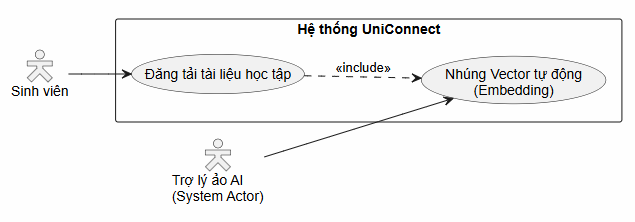
\includegraphics[width=0.85\textwidth]{Images/use-case-dang-tai-tai-lieu.png} 
    \caption{Sơ đồ Use Case Đăng tải tài liệu}
    \label{fig:usecase_dang_tai_tai_lieu}
\end{figure}

\renewcommand{\arraystretch}{1.5}
\begin{xltabular}{\textwidth}{|>{\bfseries}p{3.5cm}|X|}
    % Cấu hình Tiêu đề và Nhãn bảng
    \caption{Đặc tả Use case Đăng tải tài liệu và Nhúng tri thức} \label{tab:uc_dangtaitailieu} \\
    \hline
    \endfirsthead
    \caption[]{Đặc tả Use case Đăng tải tài liệu và Nhúng tri thức} \\
    \hline
    \endhead
    \hline
    \endfoot
    \hline
    \endlastfoot

    % Nội dung bảng
    Use case name & Đăng tải tài liệu và Nhúng tri thức (Embedding) \\ \hline
    Actor & Sinh viên, Trợ lý ảo AI (System Actor) \\ \hline
    Description & Cho phép Sinh viên đóng góp tài liệu học tập (PDF, Slide, Word) lên hệ thống. Đồng thời, hệ thống AI sẽ tự động đọc, phân tích và chuyển hóa nội dung tài liệu thành các Vector toán học để phục vụ công tác tra cứu ngữ nghĩa (Semantic Search) sau này. \\ \hline
    Preconditions & Sinh viên đã đăng nhập thành công. Tệp tin tải lên không chứa mã độc (được quét qua ở tầng Frontend/Firewall). \\ \hline
    Postconditions & Thông tin tài liệu được lưu trữ. File vật lý được lưu trữ an toàn (ví dụ: ổ cứng hoặc S3). Nội dung tài liệu được chuyển đổi thành Vector và lưu vào bảng cấu hình của cơ sở dữ liệu. \\ \hline
    
    % Phân rã Normal Flow để hỗ trợ ngắt trang
    \textbf{Normal Flow} & 1. Sinh viên truy cập vào phân hệ "Kho học liệu" và nhấn nút "Tải lên tài liệu". \\ 
    & 2. Hệ thống hiển thị biểu mẫu yêu cầu: Chọn tệp tin, Tiêu đề, Chọn Khoa/Ngành, và Gắn thẻ (Tags). \\ 
    & 3. Sinh viên đính kèm tệp và điền đầy đủ thông tin, sau đó nhấn "Đăng tải". \\ 
    & 4. Máy chủ (Backend) tiếp nhận yêu cầu, kiểm tra định dạng và kích thước tệp tin. \\ 
    & 5. Máy chủ lưu file vật lý vào hệ thống lưu trữ và tạo một bản ghi siêu dữ liệu (Metadata) vào cơ sở dữ liệu. \\ 
    & 6. Kích hoạt AI: Máy chủ đưa tác vụ đọc file vào hàng đợi. Trợ lý ảo AI (Worker) bóc tách văn bản từ file, chia nhỏ (Chunking) và gọi mô hình AI để chuyển văn bản thành Vector. \\ 
    & 7. Trợ lý AI lưu tọa độ Vector vào trường \texttt{embed} của hàng tài liệu tương ứng trong CSDL PostgreSQL. \\ 
    & 8. Hệ thống phản hồi "Đăng tải thành công" tới giao diện của Sinh viên. \\ \hline
    
    Alternative flow & Định dạng tệp không được hỗ trợ: Tại bước 3, nếu Sinh viên đính kèm các tệp thực thi (như .exe, .sh) hoặc các định dạng không phải văn bản/ảnh chuẩn, Frontend sẽ chặn lập tức và báo lỗi "Chỉ hỗ trợ tải lên định dạng PDF, DOCX, PPTX". \\ \hline
    Exception & Vượt quá dung lượng cho phép: Tại bước 4, nếu tệp tin có kích thước lớn hơn mức cấu hình hệ thống (ví dụ: lớn hơn 25MB), máy chủ sẽ từ chối xử lý luồng để bảo vệ băng thông và trả về thông báo lỗi "Dung lượng tệp vượt quá giới hạn". \\ \hline

\end{xltabular}

\subsubsection{Tương tác tài liệu}

\begin{figure}[H]
    \centering
    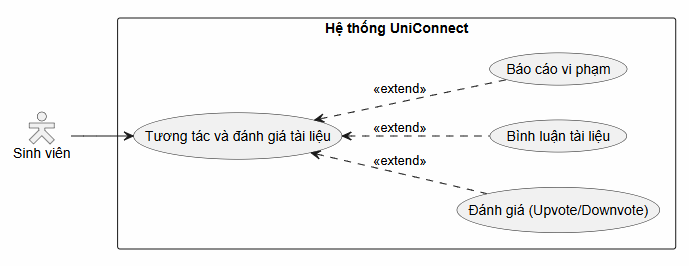
\includegraphics[width=0.85\textwidth]{Images/use-case-tuong-tac-tai-lieu.png} 
    \caption{Sơ đồ Use Case tương tác tài liệu}
    \label{fig:usecase_tuong_tac_tai_lieu}
\end{figure}

\renewcommand{\arraystretch}{1.5}
\begin{xltabular}{\textwidth}{|>{\bfseries}p{3.5cm}|X|}
    % Cấu hình Tiêu đề và Nhãn bảng
    \caption{Đặc tả Use case Tương tác tài liệu} \label{tab:uc_tuongtactailieu} \\
    \hline
    \endfirsthead
    \caption[]{Đặc tả Use case Tương tác tài liệu} \\
    \hline
    \endhead
    \hline
    \endfoot
    \hline
    \endlastfoot

    % Nội dung bảng
    Use case name & Tương tác và đánh giá tài liệu \\ \hline
    Actor & Sinh viên \\ \hline
    Description & Cho phép Sinh viên tương tác trực tiếp với các tài liệu trong kho học liệu thông qua các hành động bày tỏ quan điểm (Upvote/Downvote), để lại ý kiến thảo luận (Bình luận) hoặc gửi cảnh báo lên hệ thống khi phát hiện tài liệu có nội dung không phù hợp (Báo cáo vi phạm). \\ \hline
    Preconditions & Sinh viên đã đăng nhập thành công vào hệ thống và tài liệu mục tiêu đang ở trạng thái hiển thị công khai. \\ \hline
    Postconditions & Số lượt upvote/downvote được cập nhật, nội dung bình luận được hiển thị công khai, hoặc biểu mẫu báo cáo được chuyển tới phân hệ quản trị của Admin. \\ \hline
    
    % Phân rã Normal Flow để hỗ trợ ngắt trang
    \textbf{Normal Flow} & 1. Sinh viên chọn xem một tài liệu cụ thể trong giao diện Kho học liệu. \\ 
    & 2. Hệ thống hiển thị trang thông tin chi tiết của tài liệu, bao gồm nội dung xem trước, điểm đánh giá hiện tại, danh sách các bình luận cũ và tùy chọn báo cáo. \\ 
    & 3. Sinh viên thực hiện một trong các tương tác theo nhu cầu:
    \vspace{0.2cm}
    \begin{itemize}[leftmargin=*, noitemsep]
        \item \textbf{Nhánh Đánh giá (Upvote/Downvote):} Sinh viên nhấn vào biểu tượng tương ứng. Hệ thống ghi nhận, tính toán lại tổng điểm tài liệu và cập nhật trạng thái hiển thị của nút bấm ngay lập tức trên giao diện.
        \item \textbf{Nhánh Bình luận:} Sinh viên nhập ý kiến vào khung thảo luận và nhấn "Gửi". Hệ thống lưu dữ liệu và đưa bình luận mới vào đầu luồng hiển thị.
        \item \textbf{Nhánh Báo cáo vi phạm:} Sinh viên nhấn nút "Báo cáo", lựa chọn lý do vi phạm (tài liệu sai kiến thức, bản quyền, nội dung nhạy cảm) và nhập mô tả chi tiết, sau đó nhấn "Gửi báo cáo".
    \end{itemize} \\ 
    & 4. Hệ thống thực hiện lưu trữ các thay đổi tương ứng vào cơ sở dữ liệu và hiển thị thông báo "Thao tác thành công". \\ \hline
    
    Alternative flow & Hủy đánh giá: Ở nhánh Đánh giá, nếu Sinh viên nhấn lại vào nút bấm đang chọn (ví dụ đang Upvote và nhấn lại Upvote), hệ thống sẽ hiểu là hành động rút lại tương tác, trừ đi một điểm đánh giá và trả nút bấm về trạng thái mặc định. \\ \hline
    Exception & Tài liệu bị gỡ bỏ đột ngột: Tại bước 3, nếu tài liệu vừa bị tác giả chủ sở hữu hoặc Admin xóa/ẩn đi do vi phạm ngay tại thời điểm Sinh viên đang thao tác tương tác, Backend sẽ từ chối xử lý, trả về lỗi và Frontend hiển thị thông báo "Tài liệu này không còn tồn tại trên hệ thống". \\ \hline

\end{xltabular}

\begin{figure}[H]
    \centering
    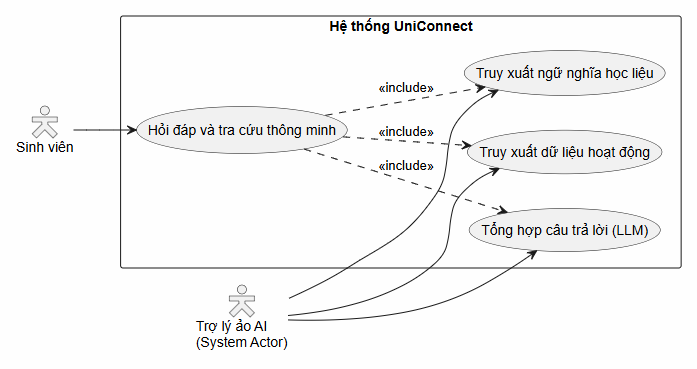
\includegraphics[width=0.85\textwidth]{Images/use-case-hoi-dap-chatbot.png} 
    \caption{Sơ đồ Use Case Hỏi đáp tri thức và tra cứu thông minh}
    \label{fig:usecase_tracuuthongminh}
\end{figure}

\renewcommand{\arraystretch}{1.5}
\begin{xltabular}{\textwidth}{|>{\bfseries}p{3.5cm}|X|}
    % Cấu hình Tiêu đề và Nhãn bảng
    \caption{Đặc tả Use case Hỏi đáp tri thức và tra cứu thông minh (RAG)} \label{tab:uc_tracuuthongminh} \\
    \hline
    \endfirsthead
    \caption[]{Đặc tả Use case Hỏi đáp tri thức và tra cứu thông minh} \\
    \hline
    \endhead
    \hline
    \endfoot
    \hline
    \endlastfoot

    % Nội dung bảng
    Use case name & Hỏi đáp tri thức và tra cứu thông minh \\ \hline
    Actor & Sinh viên, Trợ lý ảo AI (System Actor) \\ \hline
    Description & Cho phép Sinh viên đặt các câu hỏi tự nhiên về quy định nhà trường, tài liệu học thuật hoặc các hoạt động/sự kiện đang và sắp diễn ra trên bản đồ campus. Hệ thống ứng dụng kiến trúc RAG để tìm kiếm ngữ nghĩa đa nền tảng dữ liệu và phản hồi thông tin chính xác. \\ \hline
    Preconditions & Sinh viên đã đăng nhập thành công. Kho tri thức (quy chế, tài liệu) và siêu dữ liệu hoạt động (vị trí, mô tả sự kiện) đã được nhúng thành Vector và lưu trữ sẵn sàng. \\ \hline
    Postconditions & Sinh viên nhận được câu trả lời tổng hợp chính xác theo thời gian thực kèm các gợi ý liên kết (tới file tài liệu hoặc vị trí ghim sự kiện trên bản đồ). \\ \hline
    
    \textbf{Normal Flow} & 1. Sinh viên nhập câu hỏi vào khung chat (ví dụ: "Thủ tục mượn sách thư viện?" hoặc "Chiều nay ở sân thể chất có hoạt động nào không?") và nhấn gửi. \\ 
    & 2. Hệ thống tiếp nhận chuỗi văn bản và gọi mô hình Embedding để chuyển câu hỏi thành một Vector truy vấn. \\ 
    & 3. Giai đoạn phân loại và truy xuất dữ liệu hỗn hợp: Trợ lý AI thực hiện tìm kiếm khoảng cách Vector đồng thời trên các phân bảng lưu trữ của \texttt{pgvector} (bao gồm bảng phân đoạn tài liệu học liệu và bảng thông tin mô tả hoạt động). \\ 
    & 4. Trợ lý AI chọn lọc ra top các kết quả có độ tương đồng ngữ nghĩa cao nhất để làm ngữ cảnh nền tảng (Context). \\ 
    & 5. Giai đoạn tổng hợp ngữ cảnh: Hệ thống đóng gói câu hỏi gốc cùng với ngữ cảnh thu được thành một cấu trúc Prompt chuẩn mực và chuyển tiếp đến Mô hình ngôn ngữ lớn (LLM). \\ 
    & 6. LLM phân tích, tổng hợp dữ liệu và sinh ra câu trả lời bằng ngôn ngữ tự nhiên. \\ 
    & 7. Hệ thống hiển thị câu trả lời trực quan lên màn hình chat của Sinh viên (kèm đường dẫn đến điểm ghim hoạt động hoặc tệp tài liệu được nhắc tới) và lưu vào lịch sử hội thoại. \\ \hline
    
    Alternative flow & Nếu câu hỏi mang tính chất giao tiếp thông thường không chứa thực thể cần tra cứu, hệ thống bỏ qua bước truy xuất dữ liệu ở bước 3 và bước 4, chuyển trực tiếp câu hỏi sang cho LLM phản hồi theo luồng hội thoại thông thường. \\ \hline
    Exception & Tri thức nằm ngoài phạm vi hệ thống: Tại bước 3, nếu điểm số tương đồng ngữ nghĩa (Semantic Score) của tất cả các kết quả trả về từ cơ sở dữ liệu đều dưới ngưỡng an toàn cấu hình (ví dụ < 0.65), Trợ lý AI sẽ chủ động chặn luồng gửi đi của LLM nhằm chống ảo giác thông tin và đưa ra câu trả lời chuẩn: "Xin lỗi, hệ thống chưa tìm thấy thông tin phù hợp về quy định hoặc hoạt động này trong cơ sở dữ liệu." \\ \hline

\end{xltabular}

\subsubsection{Quản trị và kiểm duyệt}

\begin{figure}[H]
    \centering
    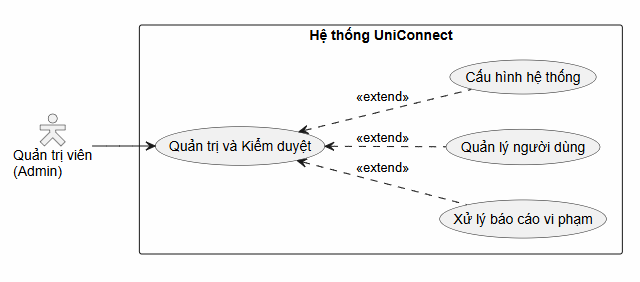
\includegraphics[width=0.85\textwidth]{Images/use-case-quan-tri.png} 
    \caption{Sơ đồ Use Case Quản trị hệ thống và Kiểm duyệt}
    \label{fig:usecase_quantri}
\end{figure}

\renewcommand{\arraystretch}{1.5}
\begin{xltabular}{\textwidth}{|>{\bfseries}p{3.5cm}|X|}
    % Cấu hình Tiêu đề và Nhãn bảng
    \caption{Đặc tả Use case Quản trị hệ thống và Kiểm duyệt} \label{tab:uc_quantri} \\
    \hline
    \endfirsthead
    \caption[]{Đặc tả Use case Quản trị hệ thống và Kiểm duyệt} \\
    \hline
    \endhead
    \hline
    \endfoot
    \hline
    \endlastfoot

    % Nội dung bảng
    Use case name & Quản trị hệ thống và Kiểm duyệt \\ \hline
    Actor & Quản trị viên (Admin) \\ \hline
    Description & Cung cấp bộ công cụ toàn diện để Admin giám sát nội dung cộng đồng, xử lý các báo cáo vi phạm từ người dùng, quản lý tài khoản và thiết lập các thông số vận hành của hệ thống. \\ \hline
    Preconditions & Admin đã xác thực thành công vào trang quản trị (Admin Dashboard) với tài khoản có quyền cao nhất. \\ \hline
    Postconditions & Các nội dung vi phạm bị gỡ bỏ, trạng thái tài khoản người dùng được cập nhật (khóa/mở), hoặc các thay đổi cấu hình được áp dụng vào cơ sở dữ liệu. \\ \hline
    
    % Phân rã Normal Flow để hỗ trợ ngắt trang
    \textbf{Normal Flow} & 1. Admin truy cập vào giao diện bảng điều khiển quản trị. \\ 
    & 2. Hệ thống hiển thị các số liệu thống kê tổng quan và danh sách các báo cáo vi phạm (Report List) đang chờ xử lý. \\ 
    & 3. Admin lựa chọn thực hiện một trong các nhánh nghiệp vụ sau:
    \vspace{0.2cm}
    \begin{itemize}[leftmargin=*, noitemsep]
        \item \textbf{Nhánh Xử lý vi phạm:} Admin xem chi tiết một báo cáo (chứa ID tài liệu hoặc hoạt động bị tố cáo). Nếu xác định vi phạm, Admin nhấn "Gỡ bỏ nội dung" và gửi cảnh cáo. Hệ thống sẽ ẩn dữ liệu này khỏi luồng hiển thị công khai.
        \item \textbf{Nhánh Quản lý người dùng:} Admin tìm kiếm một Sinh viên/Cán bộ cụ thể, thực hiện đổi vai trò (Role) hoặc nhấn "Khóa tài khoản" nếu người này vi phạm nghiêm trọng.
        \item \textbf{Nhánh Cấu hình hệ thống:} Admin điều chỉnh các danh mục dùng chung (như thêm/xóa Ngành học, Thẻ tag) hoặc cấu hình tham số hệ thống.
    \end{itemize} \\ 
    & 4. Máy chủ (Backend) ghi nhận lệnh thao tác, kiểm tra quyền JWT của Admin và thực thi thay đổi vào cơ sở dữ liệu PostgreSQL. \\ 
    & 5. Hệ thống hiển thị thông báo "Cập nhật thành công", đồng thời lưu một bản ghi nhật ký (Audit Log) về hành động vừa thực hiện để phục vụ tra soát. \\ \hline
    
    Alternative flow & Bác bỏ báo cáo: Ở nhánh Xử lý vi phạm, nếu Admin nhận thấy nội dung bị báo cáo không hề vi phạm quy định, Admin chọn "Bỏ qua báo cáo". Hệ thống sẽ đóng trạng thái của báo cáo đó mà không ảnh hưởng gì đến nội dung gốc. \\ \hline
    Exception & Xung đột dữ liệu khi kiểm duyệt: Tại bước 3, nếu nội dung vi phạm đang được xem xét đã bị tác giả tự tay xóa ngay trước đó, hệ thống sẽ báo lỗi "Nội dung này không còn tồn tại" và tự động chuyển trạng thái của báo cáo thành "Đã đóng". \\ \hline

\end{xltabular}

\subsection{Kiến trúc tổng thể hệ thống}

\begin{figure}[H]
    \centering
    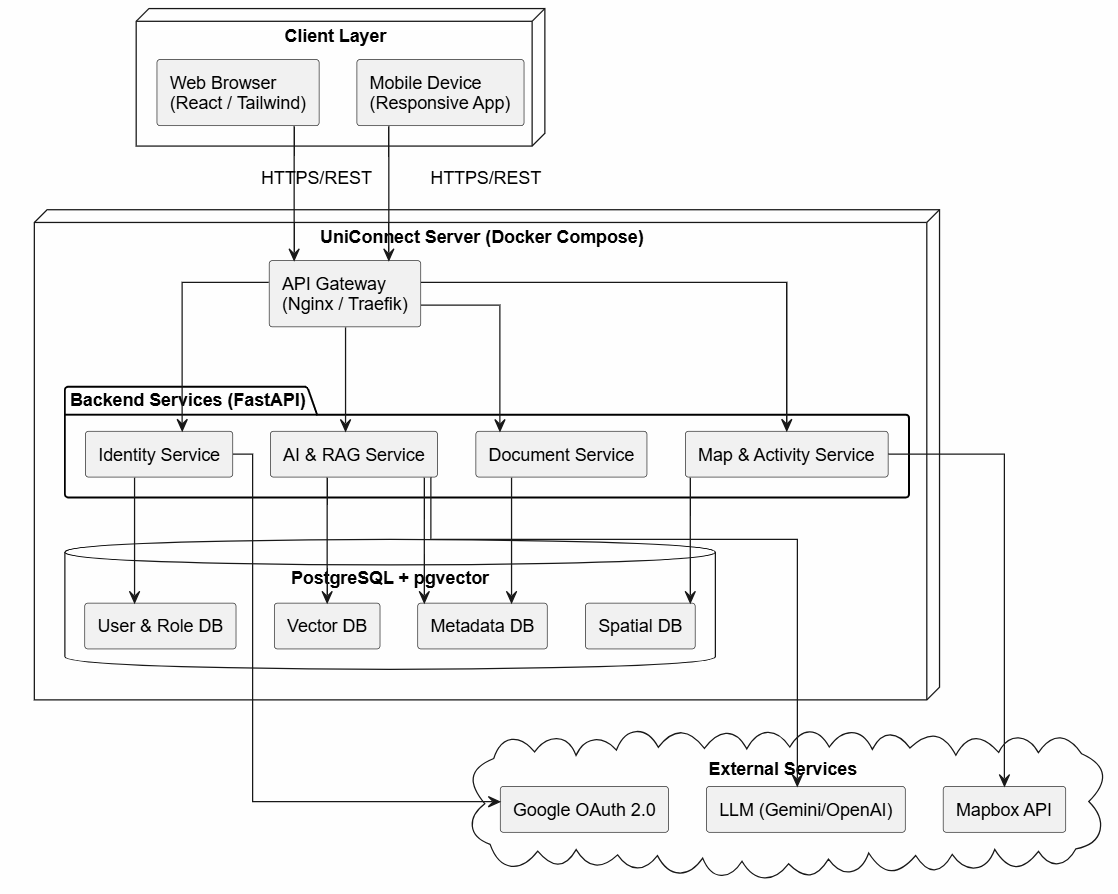
\includegraphics[width=0.85\textwidth]{Images/kien-truc-tong-the-he-thong.png} 
    \caption{Kiến trúc tổng thể hệ thống}
    \label{fig:kien_truc_tong_the_he_thong}
\end{figure}

Hệ thống UniConnect được thiết kế dựa trên kiến trúc hướng dịch vụ (Microservices), đảm bảo tính độc lập và khả năng mở rộng thông qua môi trường đóng gói container. Mọi yêu cầu từ phía Client đều đi qua API Gateway để điều hướng và kiểm soát truy cập. Về cơ chế xác thực, IdentityService tích hợp quy trình đăng nhập bảo mật, trong đó Client đảm nhiệm giao diện, còn Backend thực hiện cấp phát và xác thực JWT nội bộ qua kênh Server-to-Server, đảm bảo an toàn cho phiên làm việc. Đối với tính năng tra cứu thông minh, AI \& RAG Service đóng vai trò xử lý ngôn ngữ tự nhiên, đóng gói ngữ cảnh từ cơ sở dữ liệu Vector (pgvector) và quản lý lịch sử hội thoại trước khi gửi sang Mô hình ngôn ngữ lớn (LLM) để sinh câu trả lời. Các dịch vụ nghiệp vụ cốt lõi khác như Map \& Activity Service và Document Service hoạt động song song với phân vùng dữ liệu riêng biệt, đảm bảo sự tách biệt rõ ràng về mặt lưu trữ và logic xử lý giữa mạng xã hội bản đồ và kho học liệu.

\subsection{Mô tả mô hình thực thể kết hợp (ERD)}

\begin{figure}[H]
    \centering
    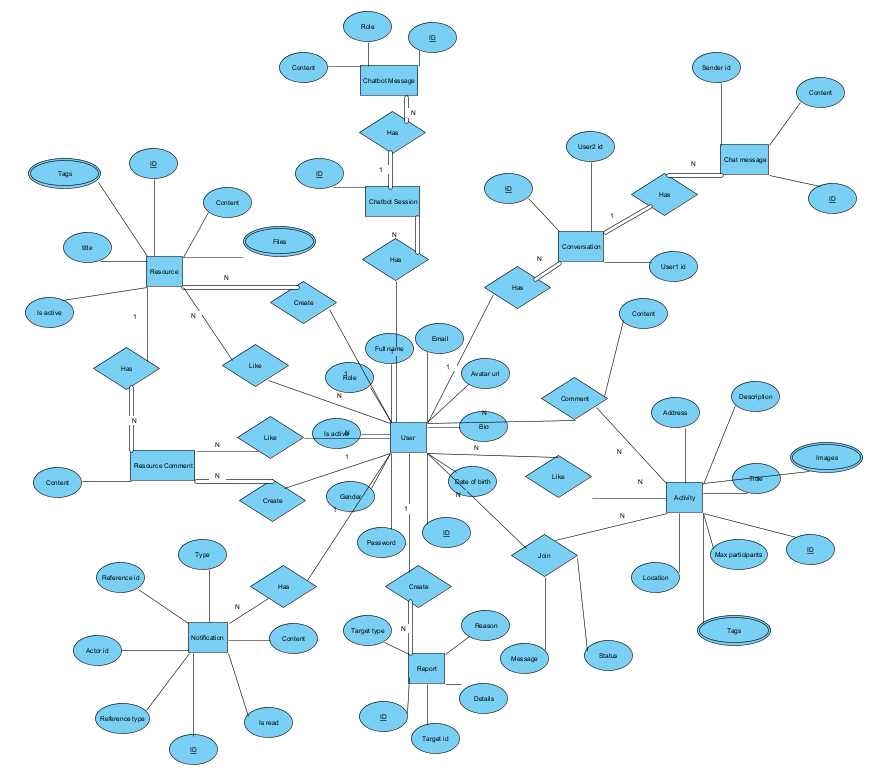
\includegraphics[width=0.85\textwidth]{Images/erd.png} 
    \caption{Entity Relationship Diagram của hệ thống}
    \label{fig:mo_hinh_erd}
\end{figure}

\subsubsection{Danh sách thực thể và thuộc tính}
\begin{enumerate}
    \item User
    Đại diện cho tất cả các tác nhân tham gia vào hệ thống UniConnect (bao gồm Sinh viên, Cán bộ trường và Quản trị viên). Thực thể này lưu trữ các thông tin cốt lõi để định danh, phân quyền và hồ sơ cá nhân của người dùng.
    \begin{itemize}
        \item ID: Mã định danh duy nhất (khóa chính), tự động tăng để quản lý người dùng.

        \item Email, Password: Thông tin tài khoản dùng để đăng nhập và mật khẩu đã được mã hóa để đảm bảo an toàn thông tin.
        
        \item Role: Vai trò của người dùng (Sinh viên, Cán bộ, hoặc Admin), quyết định quyền hạn truy cập các tính năng.
        
        \item Is Active: Trạng thái tài khoản (Cho phép hoặc Chặn truy cập).
        
        \item Full Name: Họ và tên đầy đủ của người dùng.
        
        \item Avatar URL: Đường dẫn liên kết tới hình ảnh đại diện (Lưu trữ trên Cloud hoặc Server).
        
        \item Gender, Date of Birth: Thông tin giới thiệu cơ bản về giới tính và ngày sinh.
        
        \item Bio: Đoạn giới thiệu ngắn về bản thân của người dùng.
        
        \item Created At, Updated At: (Từ TimestampMixin) Ghi lại thời điểm tạo tài khoản và lần cập nhật thông tin gần nhất.
    \end{itemize}

    \item Activity
    Thực thể này đại diện cho các sự kiện hoặc hoạt động được ghim trên bản đồ campus. Nó chứa toàn bộ thông tin về nội dung, thời gian và tọa độ địa lý để người dùng có thể tìm kiếm và tham gia.

    \begin{itemize}
        \item ID: Mã định danh duy nhất cho mỗi hoạt động.

        \item Owner ID: Khóa ngoại tham chiếu đến người tạo hoạt động (User).
        
        \item Title, Description: Tiêu đề và nội dung mô tả chi tiết về hoạt động.
        
        \item Images, Tags: Danh sách các đường dẫn ảnh minh họa và bộ thẻ từ khóa để phân loại hoạt động (ví dụ: \#thethao, \#hocthuat).
        
        \item Max Participants: Giới hạn số lượng người tham gia tối đa (nếu để trống nghĩa là không giới hạn).
        
        \item Address, Location: Địa chỉ văn bản và tọa độ địa lý thực tế (Point - vĩ độ/kinh độ). Đây là dữ liệu cốt lõi để hiển thị điểm ghim trên bản đồ.
        
        \item Start Time, End Time: Khung thời gian diễn ra hoạt động.
        
        \item Registration Deadline: Hạn chót để người dùng nhấn đăng ký tham gia.
        
        \item Auto Approve: Chế độ phê duyệt tự động. Nếu là True, người dùng nhấn tham gia sẽ vào thẳng danh sách; nếu False, chủ sở hữu phải duyệt thủ công.
        
        \item Is Active: Trạng thái hiển thị của hoạt động trên bản đồ.

        \item Created At, Updated At: (Từ TimestampMixin) Ghi lại thời điểm tạo hoạt động và lần cập nhật thông tin gần nhất.
    \end{itemize}

    \item Resource
    Thực thể này quản lý các bài viết, tài liệu học tập và tri thức được đóng góp bởi cộng đồng sinh viên hoặc cán bộ trường. Đây là nguồn dữ liệu chính để Trợ lý AI thực hiện truy xuất ngữ nghĩa.
    \begin{itemize}
        \item ID: Mã định danh duy nhất của tài liệu.

        \item Author ID: Khóa ngoại liên kết tới người đăng tải (User).
        
        \item Title: Tiêu đề của tài liệu/bài viết, giúp người dùng nhận diện nhanh nội dung.
        
        \item Content: Nội dung chi tiết của học liệu. Trường này hỗ trợ định dạng Markdown, cho phép trình bày văn bản phong phú, đính kèm hình ảnh và các liên kết tải xuống tài liệu vật lý (PDF, Slide, v.v.).
        
        \item Tags: Danh sách các từ khóa liên quan giúp phân loại và tìm kiếm tài liệu theo chủ đề hoặc môn học.
        
        \item Is Active: Trạng thái kiểm duyệt hoặc hiển thị của tài liệu trên hệ thống.

        \item Created At, Updated At: (Từ TimestampMixin) Ghi lại thời điểm tạo bài viết và lần cập nhật thông tin gần nhất.
    \end{itemize}

    \item Report
    Thực thể này quản lý các báo cáo từ người dùng đối với các nội dung khác trên hệ thống. Điểm đặc biệt của thực thể này là sử dụng cơ chế định danh mục tiêu linh hoạt, cho phép báo cáo nhiều loại đối tượng khác nhau (như hoạt động, tài liệu, hoặc bình luận).

    \begin{itemize}
        \item ID: Mã định danh duy nhất cho từng bản ghi báo cáo.

        \item Reporter ID: Khóa ngoại liên kết tới người thực hiện báo cáo (User).
        
        \item Target Type: Loại đối tượng bị báo cáo (Ví dụ: Resource, Activity, Comment). Đây là trường định danh để hệ thống biết báo cáo này thuộc phân hệ nào.
        
        \item Target ID: ID vật lý của đối tượng bị báo cáo trong bảng tương ứng của nó.
        
        \item Reason: Lý do báo cáo được chọn từ danh sách có sẵn (Ví dụ: Nội dung nhạy cảm, Thông tin sai lệch, Lừa đảo, Vi phạm bản quyền).
        
        \item Details: Nội dung mô tả chi tiết bổ sung từ người báo cáo để giúp Admin có thêm căn cứ xử lý.
        
        \item Status: Trạng thái xử lý của báo cáo (Đang chờ, Đã xử lý, hoặc Đã bác bỏ).
        
        \item Created At, Updated At: (Từ TimestampMixin) Ghi lại thời điểm tạo báo cáo và lần cập nhật thông tin gần nhất.
    \end{itemize}

    \item Notification
    Thực thể này quản lý luồng thông tin cập nhật giữa các người dùng và giữa hệ thống với người dùng. Nó đảm bảo tính tương tác thời gian thực bằng cách gửi thông điệp khi có sự thay đổi về trạng thái hoạt động hoặc các tương tác xã hội.
    \begin{itemize}
        \item ID: Mã định danh duy nhất cho mỗi thông báo.

        \item Recipient ID: (Khóa ngoại) Định danh người nhận thông báo. Đây là quan hệ bắt buộc (Total Participation).
        
        \item Actor ID: (Khóa ngoại) Định danh người gây ra hành động dẫn đến thông báo (ví dụ: người nhấn "Like" hoặc "Comment"). Trường này có thể để trống (NULL) nếu là thông báo từ hệ thống.
        
        \item Type: Phân loại thông báo dựa trên tập giá trị NotificationType (Yêu cầu tham gia, Được duyệt, Cập nhật hoạt động, Bình luận mới, Cảm xúc mới, Thông báo hệ thống).
        
        \item Reference ID \& Type: Cặp thuộc tính dùng để dẫn hướng người dùng khi nhấn vào thông báo. Reference Type xác định đối tượng liên quan (Activity, Resource, hoặc User), và Reference ID lưu ID của đối tượng đó.
        
        \item Content: Nội dung chi tiết của thông báo hiển thị cho người dùng.
        
        \item Is Read: Trạng thái kiểm soát việc người dùng đã xem thông báo hay chưa, phục vụ cho việc hiển thị dấu chấm đỏ hoặc số lượng thông báo mới trên giao diện UI.
    \end{itemize}

    \item Conversation
    Thực thể này đóng vai trò là "phòng chat" đại diện cho kênh kết nối trực tiếp giữa hai người dùng. Thay vì tạo nhiều bản ghi trùng lặp, thực thể này quản lý một cặp định danh duy nhất để duy trì lịch sử hội thoại xuyên suốt.
    \begin{itemize}
        \item ID: Mã định danh duy nhất của cuộc hội thoại.
        
        \item User1 ID \& User2 ID: Hai khóa ngoại tham chiếu đến bảng User. Hệ thống áp dụng ràng buộc UniqueConstraint và CheckConstraint ($user1\_id < user2\_id$) để đảm bảo giữa hai người dùng bất kỳ chỉ tồn tại duy nhất một phòng chat, tránh lãng phí dữ liệu.
        
        \item Last Message At: Thuộc tính lưu thời điểm tin nhắn cuối cùng được gửi. Đây là dữ liệu quan trọng để hệ thống sắp xếp (sort) danh sách hộp thư, đưa các cuộc hội thoại mới nhất lên đầu giao diện.
    \end{itemize}

    \item Chatbot session
    Thực thể này đóng vai trò là một "ngữ cảnh hội thoại" giữa người dùng và Trợ lý AI. Việc chia theo từng phiên giúp người dùng quản lý các chủ đề hỏi đáp khác nhau (ví dụ: một phiên hỏi về học phí, một phiên hỏi về sơ đồ trường) mà không bị lẫn lộn nội dung.
    \begin{itemize}
        \item ID: Mã định danh duy nhất của phiên chat.

        \item User ID: Khóa ngoại liên kết tới người sở hữu phiên chat. Một người dùng có thể có nhiều phiên hỏi đáp khác nhau.
        
        \item Title: Tiêu đề của phiên chat, thường được hệ thống tự động sinh ra từ câu hỏi đầu tiên để người dùng dễ dàng tìm lại lịch sử.
        
        \item Created At: Thời điểm bắt đầu phiên hội thoại.
    \end{itemize}

    \item Chatbot message
    Lưu trữ chi tiết từng lượt trao đổi trong một phiên chat. Đây là nguồn dữ liệu quan trọng để hệ thống "nhắc lại" ngữ cảnh cho mô hình ngôn ngữ (LLM) trong các câu hỏi tiếp theo.
    \begin{itemize}
        \item ID: Mã định danh duy nhất của tin nhắn.

        \item Session ID: Khóa ngoại liên kết chặt chẽ với phiên chat tương ứng. Khi xóa phiên chat, toàn bộ tin nhắn liên quan sẽ bị xóa theo (Cascade).

        \item Role: Vai trò của thực thể gửi tin nhắn (User - Người dùng hoặc Assistant - Trợ lý AI). Đây là thông tin bắt buộc để AI hiểu đâu là câu hỏi và đâu là câu trả lời cũ.

        \item Content: Nội dung văn bản của tin nhắn.

        \item Created At: Ghi lại thời gian để sắp xếp thứ tự các câu thoại theo đúng trình tự thời gian.
    \end{itemize}
\end{enumerate}

\subsubsection{Mô tả các mối quan hệ}

\setlist[itemize]{leftmargin=*, nosep, topsep=0pt} % Tối ưu khoảng cách trong list

\begin{longtable}{|p{0.25\textwidth}|p{0.15\textwidth}|p{0.53\textwidth}|}
    \caption{Bảng tổng hợp các mối quan hệ giữa các thực thể trong hệ thống} \label{tab:relationship_summary} \\
    
    \hline
    \textbf{Thực thể tham gia} & \textbf{Quan hệ} & \textbf{Giải thích ý nghĩa \& Ràng buộc} \\ \hline
    \endfirsthead

    \hline
    \endlastfoot

    % --- Dữ liệu bảng ---
    \textbf{User -- Activity} & \textbf{Create} \newline (1 -- N) & 
    \begin{itemize}
        \item Một \textbf{User} có thể tổ chức/quản lý nhiều \textbf{Activity}.
        \item Một \textbf{Activity} bắt buộc phải được sở hữu bởi duy nhất một \textbf{User} (Owner).
    \end{itemize} \\ \hline
    
    \textbf{User -- Activity} & \textbf{Participate} \newline (N -- N) & 
    \begin{itemize}
        \item Một \textbf{User} có thể tham gia nhiều \textbf{Activity} khác nhau.
        \item Một \textbf{Activity} có thể có nhiều người tham gia thông qua thực thể trung gian \textbf{ActivityParticipant}.
    \end{itemize} \\ \hline

    \textbf{User -- Resource} & \textbf{Create} \newline (1 -- N) & 
    \begin{itemize}
        \item Một \textbf{User} có thể đăng tải nhiều tài liệu học tập (\textbf{Resource}).
        \item Một \textbf{Resource} bắt buộc phải thuộc về một tác giả xác định.
    \end{itemize} \\ \hline

    \textbf{User -- Resource} & \textbf{Like} \newline (1 -- N) & 
    \begin{itemize}
        \item Một \textbf{User} có thể thích nhiều tài liệu học tập (\textbf{Resource}).
        \item Một \textbf{Resource} có thể được thích bởi nhiều người dùng.
    \end{itemize} \\ \hline

    \textbf{User -- Resource} & \textbf{Comment} \newline (1 -- N) & 
    \begin{itemize}
        \item Một \textbf{User} có thể bình luận trong nhiều tài liệu học tập (\textbf{Resource}).
        \item Một \textbf{Resource} có thể nhận bình luận bởi nhiều người dùng.
    \end{itemize} \\ \hline

    \textbf{Conversation -- Message} & \textbf{Has} \newline (1 -- N) & 
    \begin{itemize}
        \item Một cuộc hội thoại (\textbf{Has}) chứa nhiều tin nhắn \textbf{DirectMessage}.
        \item Một \textbf{DirectMessage} bắt buộc phải nằm trong một cuộc hội thoại cụ thể.
    \end{itemize} \\ \hline

    \textbf{User -- Chatbot Session} & \textbf{Has} \newline (1 -- N) & 
    \begin{itemize}
        \item Một \textbf{User} có thể khởi tạo nhiều phiên hỏi đáp với Trợ lý AI (\textbf{ChatSession}).
        \item Mỗi phiên chat bắt buộc gắn liền với một người dùng cụ thể.
    \end{itemize} \\ \hline

    \textbf{User -- Conversation} & \textbf{Has} \newline (1 -- N) & 
    \begin{itemize}
        \item Một \textbf{User} có thể khởi tạo nhiều phiên trò chuyện với những người dùng khác.
        \item Mỗi phiên chat bắt buộc gắn liền với một người dùng cụ thể.
    \end{itemize} \\ \hline

    \textbf{ChatSession -- Message} & \textbf{Has} \newline (1 -- N) & 
    \begin{itemize}
        \item Một phiên hỏi đáp (\textbf{ChatSession}) bao gồm nhiều lượt gửi tin nhắn \textbf{ChatMessage}.
        \item Mỗi \textbf{ChatMessage} lưu trữ nội dung hội thoại theo vai trò (User/Assistant).
    \end{itemize} \\ \hline

    \textbf{User -- Notification} & \textbf{Has} \newline (1 -- N) & 
    \begin{itemize}
        \item Một \textbf{User} có thể nhận được nhiều thông báo (\textbf{Notification}).
        \item Mỗi thông báo được gửi đích danh đến một người nhận (Recipient).
    \end{itemize} \\ \hline

    \textbf{User -- Report} & \textbf{Create} \newline (1 -- N) & 
    \begin{itemize}
        \item Một \textbf{User} có thể gửi nhiều báo cáo vi phạm (\textbf{Report}).
        \item Một báo cáo bắt buộc phải được tạo bởi một \textbf{User} xác định.
    \end{itemize} \\ \hline

    \textbf{User -- Activity comment} & \textbf{Create} \newline (1 -- N) & 
    \begin{itemize}
        \item Một \textbf{User} có thể bình luận trên các nội dung.
        \item Một bình luận được tạo bởi một người dùng cụ thể.
    \end{itemize} \\ \hline
    
    \textbf{User -- Activity comment} & \textbf{Like} \newline (N -- N) & 
    \begin{itemize}
        \item Một \textbf{User} có thể thích bình luận trong nội dung.
        \item Một bình luận hoạt động được thích bởi nhiều người dùng.
    \end{itemize} \\ \hline
\end{longtable}

\subsection{Activity diagram}

\begin{figure}[H]
    \centering
    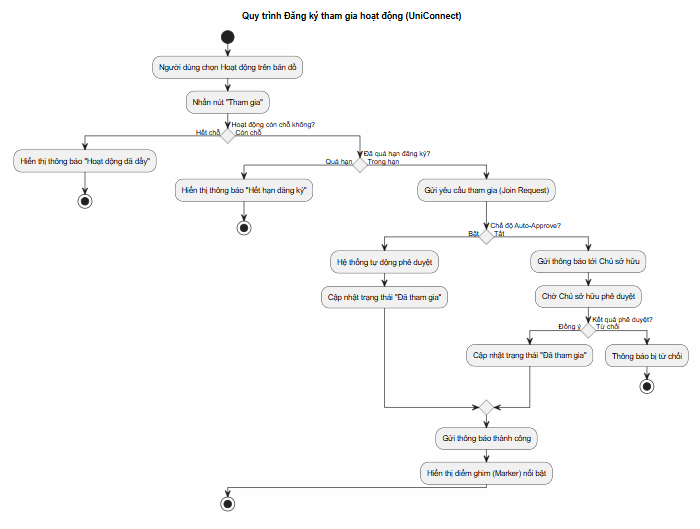
\includegraphics[width=0.85\textwidth]{Images/activity-join-activity.png} 
    \caption{Activity Diagram quy trình đăng ký tham gia hoạt động}
    \label{fig:activity_tham_gia_hoat_dong}
\end{figure}

\begin{figure}[H]
    \centering
    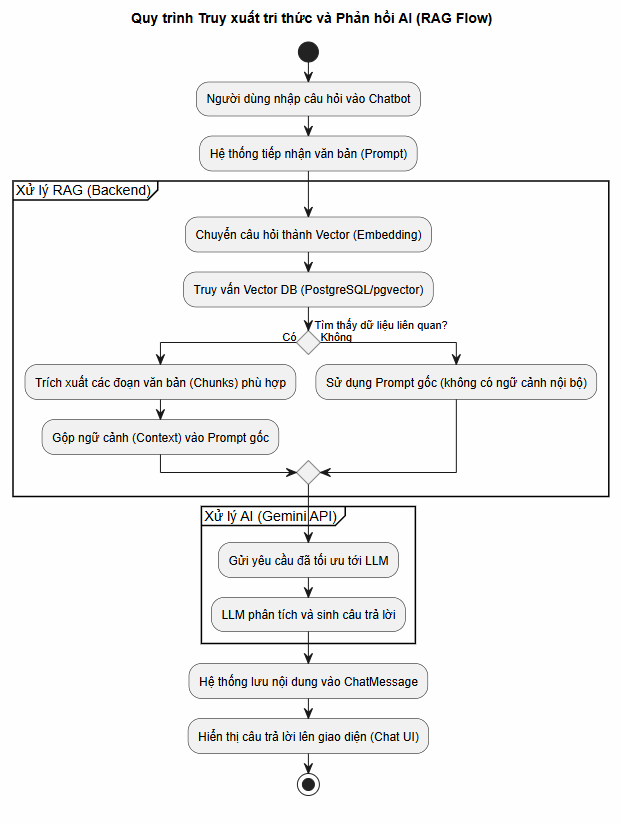
\includegraphics[width=0.85\textwidth]{Images/activity-hoi-chatbot.png} 
    \caption{Activity Diagram quy trình hỏi đáp với trợ lý AI}
    \label{fig:activity_hoi_dap_chatbot}
\end{figure}

\subsection{Sequence diagram}

\begin{figure}[H]
    \centering
    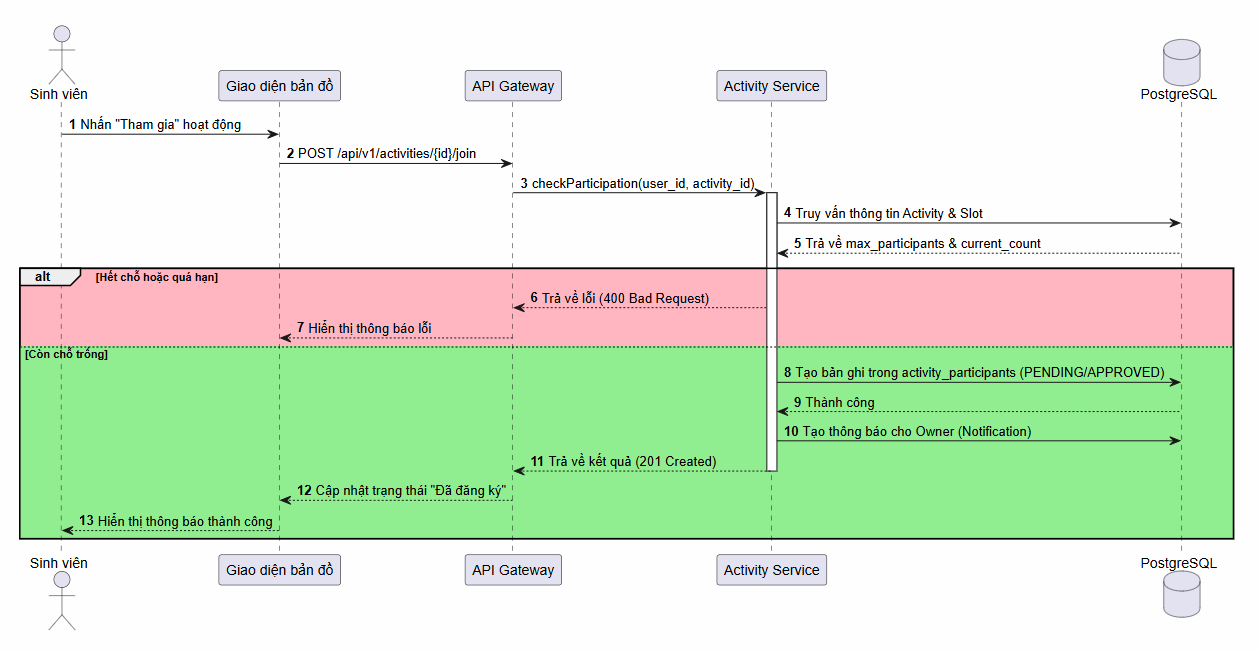
\includegraphics[width=0.85\textwidth]{Images/sequence_join_activity.png} 
    \caption{Sequence Diagram quy trình đăng ký tham gia hoạt động}
    \label{fig:sequence_tham_gia_hoat_dong}
\end{figure}

\begin{figure}[H]
    \centering
    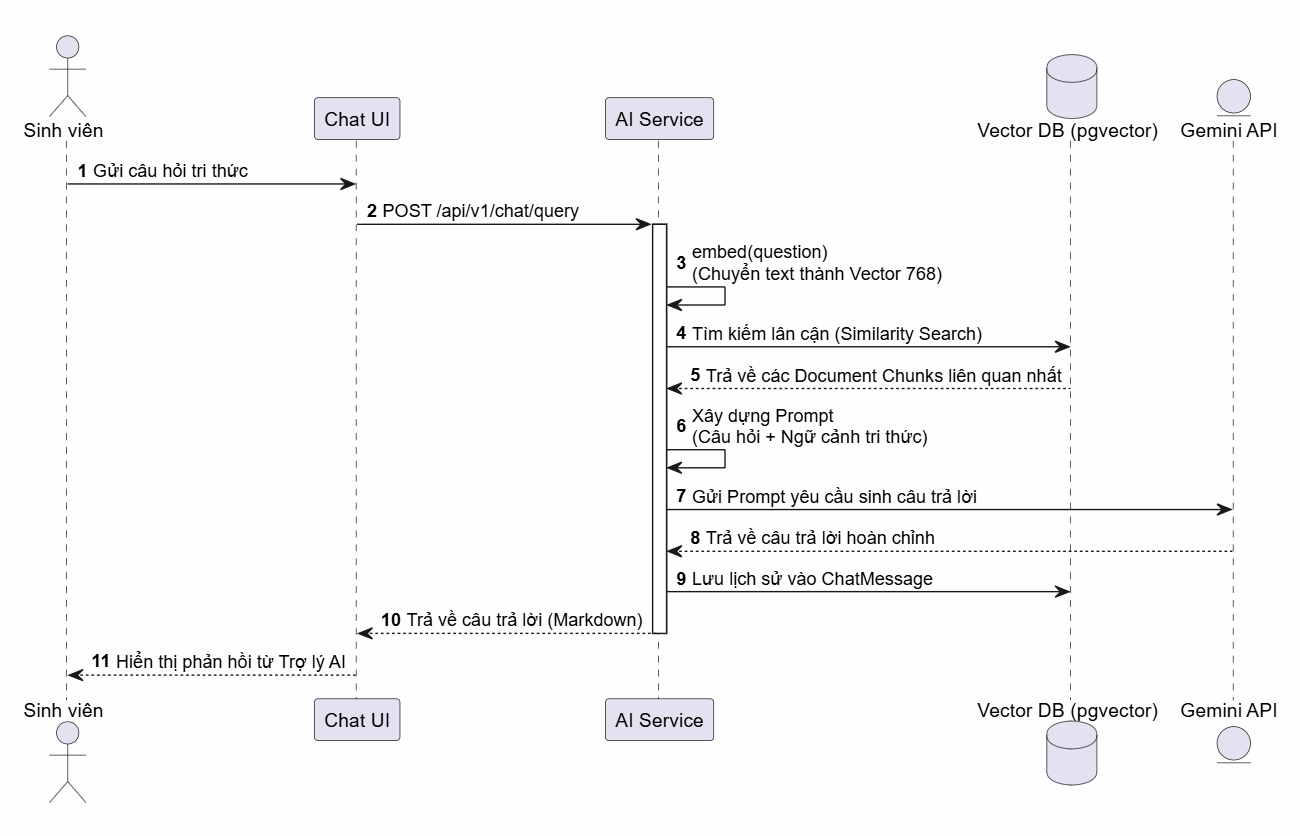
\includegraphics[width=0.85\textwidth]{Images/sequence-hoi-dap-chatbot.png} 
    \caption{Sequence Diagram quy trình hỏi đáp với trợ lý AI}
    \label{fig:sequence_hoi_dap_chatbot}
\end{figure}